\documentclass{article}
\usepackage{graphics}
\usepackage{hyperref}
\title{Freely Drawn Sketch Recognition}
\author{Denis Aleshin and Joshua Ehrlich}
\date{\today}
\begin{document}
\maketitle
\section{Description of Problem}
The problem we consider is the recognition of hand-drawn digital circuits. These circuits contain a variety of logic gates, the wires connecting these gates, and textual labels for input and output signals. Given a sketch in the form of a collection of pen strokes, we must group these strokes into shapes, while simultaneously identifying each of the shapes. An example circuit is shown in Figure \ref{fig:Circuit}.

\begin{figure}[h!]
\centering
\scalebox{.5}{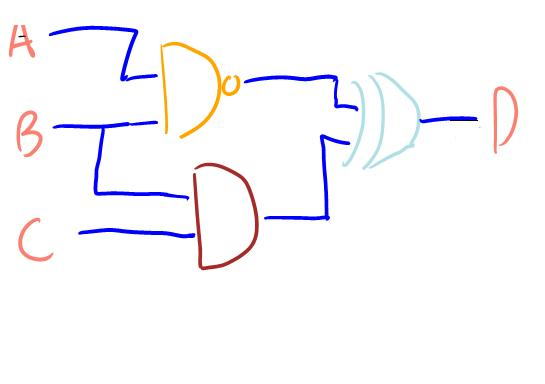
\includegraphics{CircuitComplex.JPG}}
\caption{A sample circuit, consisting of labeles 'A'-'D', wires, and a NAND, AND and XOR gate.}
\label{fig:Circuit}
\end{figure}

In previous attempts, recognition was a linear proccess. First the strokes were separately classified as either wire, label or gate. Then these classifications would be used to group the strokes into shapes. Finally, the shapes would be recognized as specific gates, inputs and outputs. This sequence is presented visually in Figure \ref{fig:Sequence}. Unfortunately, it is difficult to classify strokes when they are taken out of context, even when many features are used. The errors of classification propogate through the linear approach to make mistakes common.

\begin{figure}[h!]
\centering
\scalebox{1}{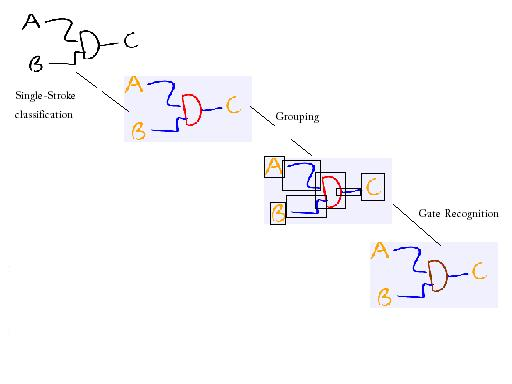
\includegraphics{Sequence.JPG}}
\caption{A visual representation of linear recognition. Strokes are classified individually (red for gate, blue for wire and orange for label). Then they are grouped, and finally the gate group is identified as an AND gate.}
\label{fig:Sequence}
\end{figure}

We focused on the question of using context, derived from the result of linear recognition, to improve grouping and recognition results. The use of context is essential to the problem of circuit recognition. In Figure \ref{fig:Circuit}, for example, it is difficult to distinguish between the AND gate and the label 'D' if one ignores their connection to the rest of the diagram.
\section{Using a Bayes Classifier for Adding Context to Recognition}
\subsection{Background}
One way to distinguish between an AND gate and the label 'D' is to note that a label should connect to only one wire, and a gate should connect to one wire on one side, and two or more on the other.

Finding the connections between different shapes in a sketch and using their contextual information can help us with both the grouping and recognition steps of the proccess.
\subsection{Design}
In order to take advantage of context, we implemented a Naive Bayes network. A Bayes network finds the best explanation for observed data by combining conditional probabilities of features of the data. In our case the data is the sketch, and the explanation is the proper identification of each part of the sketch.

A Naive Bayes network is the simplest type of Bayes network. We build one of these networks for each shape. There is one parent node, which in our case is the classification of the shape, and the multiple children nodes, which represent the features of the observed data.

We can use Bayes rule in combination with the assumption that the features are independent (given the classification of the shape) to produce the following equation:
\[
P(c_i\ |\ f_1,\ f_2,\ f_3) = \alpha P(f_1\ |\ c_i) P(f_2\ |\ c_i) P(f_3\ |\ c_i)P(c_i)
\]

On the left side we see our desired quantity: the probability of a given classification ($c_i$) given the observed features ($f_1, f_2, f_3$). The conditional probabilities on the right hand side are much easier to extract from our data. For example, we can compute the probability that we detect a shape touching 3 or more wires given that it is an AND gate.

We used three features to construct our bayes network. The first was the number of strokes in the given shape. The second feature was the result of the linear recognition proccess. Finally, the third feature was the way that the given shape was connected to the rest of the sketch.

In order to determine connections, we looked at the endpoints of every wire. We found the direction of the wire at the endpoint, and found the closest shape in the given direction. In doing this, we made the assumption that every wire makes exactly two connections. For certain other shapes, different connections were detected. NOTBUBBLES connected to the two closest shapes, and labelboxes checked for contained shapes.
\subsection{Results}

We tested the classifier on labeled data trying to see how much incorporating the connection information helped.  We present here the confusion matrix for this classifier.  Although it has some weak points, most of the errors occur between classes with similar connection information.  In addition these errors are similar to the errors in the original classifier.
\begin{center}
\begin{tabular}{|c|l|c|c|c|c|c|c|c|c|c|c|}
\hline
&&\multicolumn{9}{c}{ACTUAL LABEL}\\
\hline
&&\tiny{AND}&\tiny{LABEL}&\tiny{LABELBOX}&\tiny{NAND}&\tiny{NOR}&\tiny{NOT}&\tiny{NOTBUBBLE}&\tiny{OR}&\tiny{WIRE}&\tiny{XOR}\\
\hline
P&\tiny{AND}&.81&0&0&.22&0&.04&0&.28&0&0\\
R&\tiny{LABEL}&.09&.93&.03&0&0&.04&0&.07&.03&0\\
E&\tiny{LABELBOX}&0&0&.97&0&0&0&0&0&0&0\\
D&\tiny{NAND}&.02&0&0&.28&0&0&0&0&0&0\\
I&\tiny{NOR}&0&0&0&.06&.37&.01&0&0&.03&.06\\
C&\tiny{NOT}&0&.02&0&.06&.16&.82&0&0&.02&0\\
T&\tiny{NOTBUBBLE}&.02&.01&0&0&0&0&.83&0&.01&0\\
E&\tiny{OR}&.0&.01&0&.39&.21&.01&0&.61&.01&.13\\
D&\tiny{WIRE}&.02&.02&0&0&0&0&.17&.02&.88&0\\
&\tiny{XOR}&0&.02&0&0&.26&.01&0&.03&.02&.81\\
\hline
\end{tabular}
\end{center}


\begin{center}
\begin{tabular}{|c|l|c|c|c|c|c|c|c|c|c|}
\hline
&&\multicolumn{9}{c}{ACTUAL LABEL}\\
\hline
&&\tiny{AND}&\tiny{LABEL}&\tiny{LABELBOX}&\tiny{NAND}&\tiny{NOR}&\tiny{NOT}&\tiny{NOTBUBBLE}&\tiny{OR}&\tiny{XOR}\\
\hline
P&\tiny{AND}       &.75&  0&.22&.22&.1 &.28&.1 &.17&0  \\
R&\tiny{LABEL}     &0  &1  &0  &0  &0  &0  &0  &0  &0  \\
E&\tiny{LABELBOX}  &.03&0  &.42&0  &.05&.03&.07&.05&.01\\
D&\tiny{NAND}      &.11&0  &.07&.28&0  &.42&.08&.01&.01\\
I&\tiny{NOR}       &.02&0  &.04&.06&.55&.11&.17&.11&.05\\
C&\tiny{NOT}       &.05&0  &.07&.06&.13&.14&.46&.12&.12\\
T&\tiny{NOTBUBBLE} &.01&0  &.01&0  &0  &0  &.05&.01&0  \\
E&\tiny{OR}        &.02&0  &.16&.39&.13&.01&.05&.34&.1 \\
D&\tiny{XOR}       &.01&0  &.01&0  &.04&.01&.02&.19&.71\\
\hline
\end{tabular}
\end{center}
Comparing this classifier with the original classifier indicates that there is an advantage gained by using the connection information.  However, more detailed features will be needed to make significant improvements.
\end{document}
